\documentclass[a4paper,AutoFakeBold,AutoFakeSlant]{ctexart}
\usepackage[a4paper,left=3cm,right=3cm,top=2.5cm,bottom=2.5cm]{geometry}
\usepackage{graphicx}
\usepackage{pythonhighlight}
\usepackage[mathscr]{eucal}
\usepackage{mathrsfs}
\usepackage{booktabs}
\usepackage{capt-of} 
\usepackage{hyperref} 
\usepackage{abstract}
\usepackage{amsmath}
\usepackage{listings}
\usepackage{color}
\definecolor{gray}{rgb}{0.5,0.5,0.5}
\definecolor{dkgreen}{rgb}{.068,.578,.068}
\definecolor{dkpurple}{rgb}{.320,.064,.680}

\renewcommand{\abstractname}{}    % clear the title
\renewcommand{\absnamepos}{empty}
%去除摘要两边缩进
\makeatletter
  \renewenvironment{abstract}{%
      \if@twocolumn
        \section*{\abstractname}%
      \else
        \small
        \begin{center}%
          {\bfseries \abstractname\vspace{-.5em}\vspace{\z@}}%
        \end{center}%
      \fi}
      {}
  \makeatother
  \lstset{
    language=Matlab,
    keywords={break,case,catch,continue,else,elseif,end,for,function,
       global,if,otherwise,persistent,return,switch,try,while},
    basicstyle=\ttfamily,
    keywordstyle=\color{blue}\bfseries,
    commentstyle=\color{dkgreen},
    stringstyle=\color{dkpurple},
    backgroundcolor=\color{white},
    tabsize=4,
    showspaces=false,
    showstringspaces=false
 }




\title{\heiti{第一次作业}}
\author{PB19151769~~~~~~马宇骁}

\begin{document}

\maketitle

\begin{abstract}\zihao{-4} \kaishu
\noindent 
\textbf{\heiti 摘要:}高空抛物严重威胁着人们的生命安全。2021 年 3 月 1 日,高空抛物罪正式入刑。现在,假设一个
质量为 m 的物体从高度 h 处自由落下,砸在地面上。物体对于地面的冲击力显然依赖于物
体和地面的性质,例如冰雹 vs 细雨、水泥地面 vs 泥水地面。本文将建立数学模型,定量分析
在各种情形下物体对于地面的破坏程度。\cite{《数学建模(第五版)》}
   \newline
\textbf{\heiti 关键词:}高空抛物、地面破坏程度
\end{abstract}


\section{背景}

高空抛物罪是中华人民共和国的一个独立刑事罪名,若有人从建筑物或者其他高空处抛掷物品,造成人身或财产伤害后果,将处一年以下有期徒刑并缴纳罚款。\cite{高空抛物罪首案的警示意义}

仅仅依靠《侵权责任法》来进行处理,很难切实保障人民群众的安全,此次《刑法》修正案十一新设了高空抛物罪,明确了定罪和量刑,能够准确地追究高空抛物行为人的责任,起到了法律的威慑作用。


\section{问题分析}

根据题目的内容说明,从高度h处自由落下,因此属于竖直方向的抛物的运动。因此不考虑横向的分力对于模型运动的影响。

理想中,高空抛物是自由落体,但考虑实际的情况,不失一般性,需要考虑空气阻力。
与此同时,在物体触底时,动量的变化,物体的刚性,地面的材料等都会对结果产生影响。

\section{模型}

\subsection{模型假设}
1.物体质量m从h处竖直落下;

2.物体在运动过程中质量不变;

3.空气阻力由经验为:

\qquad $ f = \frac{1}{2}c\rho Sv^2 $;

4.受力只有向下重力和向上空气阻力;

5.向下为正方向。

\subsection{模型建立}
\subsubsection{符号体系}
\begin{table}[htbp]
\begin{center}
\setlength{\tabcolsep}{15mm}{
\begin{tabular}{ccc}
  \toprule
    字母 & 单位 & 解释\\
  \midrule
  \hline
  $ m $ & $ kg $ & 物体质量  \\
  \hline
  $ t $ & $ s $ & 时间  \\ 
  \hline
  $ v $ & $ m/s $ & 速度 \\  
  \hline
  $ g $ & $ m/s^2 $ & 重力加速度 \\  
  \hline
  $ a $ & $ m/s^2 $ & 加速度  \\  
  \hline
  $ h $ & $ m $ & 高度  \\  
  \hline
  $ x $ & $ m $ & 下落距离  \\    
  \hline
  $ c $ & $ - $ & 空气阻力系数  \\  
  \hline
  $ \rho $ & $ kg/m^3 $ & 密度  \\  
  \hline
  $ S $ & $ m^2 $ & 迎风面积  \\  
  \hline
  $ f $ & $ N $ & 空气阻力  \\  
  \hline
  $ P $ & $ Pa $ & 对地压强  \\  
\hline
\bottomrule
\end{tabular}}
\end{center}
\end{table}

\subsubsection{推导}
为方便推导,令$ k = \frac{1}{2}c\rho S $作为比例系数,此时,

\begin{equation}
  f = kv^2
\end{equation}
由牛顿第二定律有,
\begin{equation}
  mg - f = ma
\end{equation}
由(1) (2)和加速度定义可知,
\begin{equation}
  mg - k(\frac{dx}{dt})^2 = m\frac{d^2 x}{dt^2}
\end{equation}
由从静止开始,即$ x'(0) = 0, x(0) = 0 $解得微分方程(3)得到下落距离的函数:
\begin{equation}
  x(t) = \frac{m*ln(cosh(\sqrt{\frac{kg}{m}}t))}{k}
\end{equation}
速度函数:
\begin{equation}
  v(t) = \sqrt{\frac{gm}{k}} tanh(\sqrt{\frac{kg}{m}}t)
\end{equation}
由(4)式,$ x(t) = h $时,落地$t_1$为,
\begin{equation}
  t_1 = \frac{\sqrt{m} cosh^{-1}(e^{\frac{kh}{m}})}{\sqrt{gk}}
\end{equation}
带入(5)可知最终的速度为:
\begin{equation}
  v_1 = \sqrt{\frac{gm}{k}} tanh(cosh^{-1}(e^{\frac{kh}{m}}))
\end{equation}
由动量定理可以推出触地时有,
\begin{equation}
  F = \frac{mv_1}{\Delta t} = \frac{m\sqrt{\frac{gm}{k}} tanh(cosh^{-1}(e^{\frac{kh}{m}}))}{\Delta t}
\end{equation}
\begin{equation}
  P = \frac{mv_1}{\Delta t S} = \frac{m\sqrt{\frac{gm}{k}} tanh(cosh^{-1}(e^{\frac{kh}{m}}))}{\Delta t S}
\end{equation}
不妨根据实际的一般情况下的数据,取$ m = 0.00005 kg $,$ g = 9.8 m/s^2 $,$ k = \frac{1}{2}c\rho S = 0.5*0.5*1.3*6.6*10^{-3} = 2.13*10^{-3} $,带入得到:
\begin{equation}
  P = \frac{mv_1}{\Delta tS} = \frac{2.398*10^{-5} tanh(cosh^{-1}(e^{42.6h}))}{\Delta t * 6.6*10^{-3}} Pa
\end{equation}
用\textsc{MATLAB}作图得到:
\begin{center}
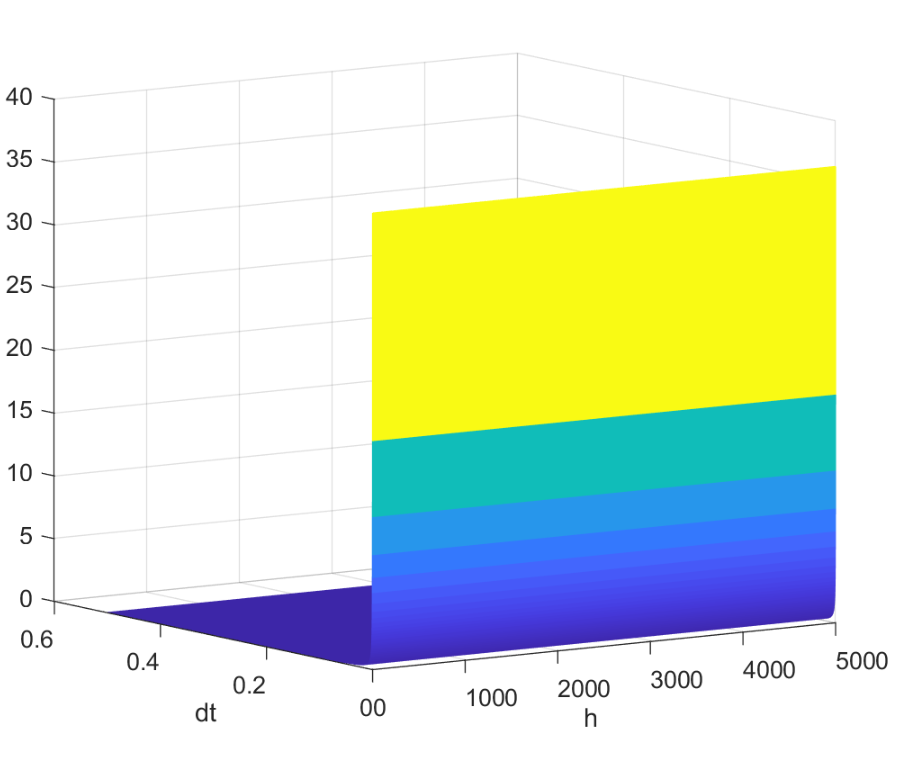
\includegraphics[scale=0.3]{1.png}
\end{center}


\subsection{模型结论}
由P的最终表达式和图像可以看出,给定高度越高,触地时间越短。最终带给地面的压强越大。

当$ h $给定为1km时,题中的物体的分析如下:
\begin{itemize}
  \item[·] $\Delta t = 0.01s$
  \item[] $ P = 0.3633 Pa $
\end{itemize}
\begin{itemize}
  \item[·] $\Delta t = 0.0001s$
  \item[] $ P = 36.3333 Pa $
\end{itemize}
由此,

\begin{itemize}
  \item[*] 冰雹
  \begin{itemize} 
    \item[·] 水泥
    \item[] $\Delta t$触地时间短,P较大,对地面的破坏程度取决于地面具体强度可能会砸出小凹痕。
    \item[·] 泥水
    \item[] $\Delta t$触地时间稍长,P较小,能砸出较大明显的坑并溅出。
  \end{itemize} 
\end{itemize}

\begin{itemize}
  \item[*] 细雨
  \begin{itemize} 
    \item[·] 水泥
    \item[] $\Delta t$触地时间长,P小,对地面的破坏程度物理角度基本没有影响。
    \item[·] 泥水
    \item[] $\Delta t$触地时间长,P很小,可能落下位置稍有小凹陷但基本没有影响。
  \end{itemize} 
\end{itemize}

模型简洁,能够方便想要快速了解天气中的抛物对于地面影响的学生有一个初步的概念,便于后续学习和掌握更复杂的模型打下一个良好的思想基础。


\subsection{模型问题}
\begin{itemize}
  \item[*] 测量问题

1.触地的$ \Delta t $的具体数据难以测量;

2.当地的空气阻力系数c难以精准测出;

3.地面的强度的具体数据难以测出。
\end{itemize}
\begin{itemize}
  \item[*] 客观问题

1.空气不是完全静止(有风),导致空气阻力不是理想中竖直向上;

2.冰雹/细雨下落时会因为摩擦蒸发等原因损失质量,导致m不是定值。
\end{itemize}

以上问题可能会使得模型的估计产生偏差。

\section*{代码附录}
\textsc{MATLAB}程序显示如下:
\begin{lstlisting}[frame=single]
h = 1:5000;
t = 1:5000;
t = t/10000;
% 因变量
xlen = length(h);
ylen = length(t);
P = zeros(ylen,xlen);
for i = 1:xlen
for j = 1:ylen
P(j,i) = (0.00002398*tanh(acosh(exp(42.6*h(i)))))/(t(j)*0.0066);
end
end
[xx,yy]=meshgrid(h,t);
figure;mesh(xx,yy,F)
xlabel('h');ylabel('dt');zlabel('P');

view([-34.500 9.303])
\end{lstlisting}

\bibliographystyle{ieeetr}
\bibliography{bibl}

\end{document}
